
%% bare_conf.tex
%% V1.3
%% 2007/01/11
%% by Michael Shell
%% See:
%% http://www.michaelshell.org/
%% for current contact information.
%%
%% This is a skeleton file demonstrating the use of IEEEtran.cls
%% (requires IEEEtran.cls version 1.7 or later) with an IEEE conference paper.
%%
%% Support sites:
%% http://www.michaelshell.org/tex/ieeetran/
%% http://www.ctan.org/tex-archive/macros/latex/contrib/IEEEtran/
%% and
%% http://www.ieee.org/

%%*************************************************************************
%% Legal Notice:
%% This code is offered as-is without any warranty either expressed or
%% implied; without even the implied warranty of MERCHANTABILITY or
%% FITNESS FOR A PARTICULAR PURPOSE! 
%% User assumes all risk.
%% In no event shall IEEE or any contributor to this code be liable for
%% any damages or losses, including, but not limited to, incidental,
%% consequential, or any other damages, resulting from the use or misuse
%% of any information contained here.
%%
%% All comments are the opinions of their respective authors and are not
%% necessarily endorsed by the IEEE.
%%
%% This work is distributed under the LaTeX Project Public License (LPPL)
%% ( http://www.latex-project.org/ ) version 1.3, and may be freely used,
%% distributed and modified. A copy of the LPPL, version 1.3, is included
%% in the base LaTeX documentation of all distributions of LaTeX released
%% 2003/12/01 or later.
%% Retain all contribution notices and credits.
%% ** Modified files should be clearly indicated as such, including  **
%% ** renaming them and changing author support contact information. **
%%
%% File list of work: IEEEtran.cls, IEEEtran_HOWTO.pdf, bare_adv.tex,
%%                    bare_conf.tex, bare_jrnl.tex, bare_jrnl_compsoc.tex
%%*************************************************************************

% *** Authors should verify (and, if needed, correct) their LaTeX system  ***
% *** with the testflow diagnostic prior to trusting their LaTeX platform ***
% *** with production work. IEEE's font choices can trigger bugs that do  ***
% *** not appear when using other class files.                            ***
% The testflow support page is at:
% http://www.michaelshell.org/tex/testflow/



% Note that the a4paper option is mainly intended so that authors in
% countries using A4 can easily print to A4 and see how their papers will
% look in print - the typesetting of the document will not typically be
% affected with changes in paper size (but the bottom and side margins will).
% Use the testflow package mentioned above to verify correct handling of
% both paper sizes by the user's LaTeX system.
%
% Also note that the "draftcls" or "draftclsnofoot", not "draft", option
% should be used if it is desired that the figures are to be displayed in
% draft mode.
%
\documentclass[conference]{IEEEtran}
% Add the compsoc option for Computer Society conferences.
%
% If IEEEtran.cls has not been installed into the LaTeX system files,
% manually specify the path to it like:
% \documentclass[conference]{../sty/IEEEtran}





% Some very useful LaTeX packages include:
% (uncomment the ones you want to load)


% *** MISC UTILITY PACKAGES ***
%
%\usepackage{ifpdf}
% Heiko Oberdiek's ifpdf.sty is very useful if you need conditional
% compilation based on whether the output is pdf or dvi.
% usage:
% \ifpdf
%   % pdf code
% \else
%   % dvi code
% \fi
% The latest version of ifpdf.sty can be obtained from:
% http://www.ctan.org/tex-archive/macros/latex/contrib/oberdiek/
% Also, note that IEEEtran.cls V1.7 and later provides a builtin
% \ifCLASSINFOpdf conditional that works the same way.
% When switching from latex to pdflatex and vice-versa, the compiler may
% have to be run twice to clear warning/error messages.






% *** CITATION PACKAGES ***
%
%\usepackage{cite}
% cite.sty was written by Donald Arseneau
% V1.6 and later of IEEEtran pre-defines the format of the cite.sty package
% \cite{} output to follow that of IEEE. Loading the cite package will
% result in citation numbers being automatically sorted and properly
% "compressed/ranged". e.g., [1], [9], [2], [7], [5], [6] without using
% cite.sty will become [1], [2], [5]--[7], [9] using cite.sty. cite.sty's
% \cite will automatically add leading space, if needed. Use cite.sty's
% noadjust option (cite.sty V3.8 and later) if you want to turn this off.
% cite.sty is already installed on most LaTeX systems. Be sure and use
% version 4.0 (2003-05-27) and later if using hyperref.sty. cite.sty does
% not currently provide for hyperlinked citations.
% The latest version can be obtained at:
% http://www.ctan.org/tex-archive/macros/latex/contrib/cite/
% The documentation is contained in the cite.sty file itself.






% *** GRAPHICS RELATED PACKAGES ***
%
\ifCLASSINFOpdf
   \usepackage[pdftex]{graphicx}
  % declare the path(s) where your graphic files are
  % \graphicspath{{../pdf/}{../jpeg/}}
  % and their extensions so you won't have to specify these with
  % every instance of \includegraphics
  % \DeclareGraphicsExtensions{.pdf,.jpeg,.png}
\else
  % or other class option (dvipsone, dvipdf, if not using dvips). graphicx
  % will default to the driver specified in the system graphics.cfg if no
  % driver is specified.
  % \usepackage[dvips]{graphicx}
  % declare the path(s) where your graphic files are
  % \graphicspath{{../eps/}}
  % and their extensions so you won't have to specify these with
  % every instance of \includegraphics
  % \DeclareGraphicsExtensions{.eps}
\fi
% graphicx was written by David Carlisle and Sebastian Rahtz. It is
% required if you want graphics, photos, etc. graphicx.sty is already
% installed on most LaTeX systems. The latest version and documentation can
% be obtained at: 
% http://www.ctan.org/tex-archive/macros/latex/required/graphics/
% Another good source of documentation is "Using Imported Graphics in
% LaTeX2e" by Keith Reckdahl which can be found as epslatex.ps or
% epslatex.pdf at: http://www.ctan.org/tex-archive/info/
%
% latex, and pdflatex in dvi mode, support graphics in encapsulated
% postscript (.eps) format. pdflatex in pdf mode supports graphics
% in .pdf, .jpeg, .png and .mps (metapost) formats. Users should ensure
% that all non-photo figures use a vector format (.eps, .pdf, .mps) and
% not a bitmapped formats (.jpeg, .png). IEEE frowns on bitmapped formats
% which can result in "jaggedy"/blurry rendering of lines and letters as
% well as large increases in file sizes.
%
% You can find documentation about the pdfTeX application at:
% http://www.tug.org/applications/pdftex





% *** MATH PACKAGES ***
%
%\usepackage[cmex10]{amsmath}
% A popular package from the American Mathematical Society that provides
% many useful and powerful commands for dealing with mathematics. If using
% it, be sure to load this package with the cmex10 option to ensure that
% only type 1 fonts will utilized at all point sizes. Without this option,
% it is possible that some math symbols, particularly those within
% footnotes, will be rendered in bitmap form which will result in a
% document that can not be IEEE Xplore compliant!
%
% Also, note that the amsmath package sets \interdisplaylinepenalty to 10000
% thus preventing page breaks from occurring within multiline equations. Use:
%\interdisplaylinepenalty=2500
% after loading amsmath to restore such page breaks as IEEEtran.cls normally
% does. amsmath.sty is already installed on most LaTeX systems. The latest
% version and documentation can be obtained at:
% http://www.ctan.org/tex-archive/macros/latex/required/amslatex/math/





% *** SPECIALIZED LIST PACKAGES ***
%
%\usepackage{algorithmic}
% algorithmic.sty was written by Peter Williams and Rogerio Brito.
% This package provides an algorithmic environment fo describing algorithms.
% You can use the algorithmic environment in-text or within a figure
% environment to provide for a floating algorithm. Do NOT use the algorithm
% floating environment provided by algorithm.sty (by the same authors) or
% algorithm2e.sty (by Christophe Fiorio) as IEEE does not use dedicated
% algorithm float types and packages that provide these will not provide
% correct IEEE style captions. The latest version and documentation of
% algorithmic.sty can be obtained at:
% http://www.ctan.org/tex-archive/macros/latex/contrib/algorithms/
% There is also a support site at:
% http://algorithms.berlios.de/index.html
% Also of interest may be the (relatively newer and more customizable)
% algorithmicx.sty package by Szasz Janos:
% http://www.ctan.org/tex-archive/macros/latex/contrib/algorithmicx/




% *** ALIGNMENT PACKAGES ***
%
%\usepackage{array}
% Frank Mittelbach's and David Carlisle's array.sty patches and improves
% the standard LaTeX2e array and tabular environments to provide better
% appearance and additional user controls. As the default LaTeX2e table
% generation code is lacking to the point of almost being broken with
% respect to the quality of the end results, all users are strongly
% advised to use an enhanced (at the very least that provided by array.sty)
% set of table tools. array.sty is already installed on most systems. The
% latest version and documentation can be obtained at:
% http://www.ctan.org/tex-archive/macros/latex/required/tools/


%\usepackage{mdwmath}
%\usepackage{mdwtab}
% Also highly recommended is Mark Wooding's extremely powerful MDW tools,
% especially mdwmath.sty and mdwtab.sty which are used to format equations
% and tables, respectively. The MDWtools set is already installed on most
% LaTeX systems. The lastest version and documentation is available at:
% http://www.ctan.org/tex-archive/macros/latex/contrib/mdwtools/


% IEEEtran contains the IEEEeqnarray family of commands that can be used to
% generate multiline equations as well as matrices, tables, etc., of high
% quality.


%\usepackage{eqparbox}
% Also of notable interest is Scott Pakin's eqparbox package for creating
% (automatically sized) equal width boxes - aka "natural width parboxes".
% Available at:
% http://www.ctan.org/tex-archive/macros/latex/contrib/eqparbox/





% *** SUBFIGURE PACKAGES ***
%\usepackage[tight,footnotesize]{subfigure}
% subfigure.sty was written by Steven Douglas Cochran. This package makes it
% easy to put subfigures in your figures. e.g., "Figure 1a and 1b". For IEEE
% work, it is a good idea to load it with the tight package option to reduce
% the amount of white space around the subfigures. subfigure.sty is already
% installed on most LaTeX systems. The latest version and documentation can
% be obtained at:
% http://www.ctan.org/tex-archive/obsolete/macros/latex/contrib/subfigure/
% subfigure.sty has been superceeded by subfig.sty.



%\usepackage[caption=false]{caption}
%\usepackage[font=footnotesize]{subfig}
% subfig.sty, also written by Steven Douglas Cochran, is the modern
% replacement for subfigure.sty. However, subfig.sty requires and
% automatically loads Axel Sommerfeldt's caption.sty which will override
% IEEEtran.cls handling of captions and this will result in nonIEEE style
% figure/table captions. To prevent this problem, be sure and preload
% caption.sty with its "caption=false" package option. This is will preserve
% IEEEtran.cls handing of captions. Version 1.3 (2005/06/28) and later 
% (recommended due to many improvements over 1.2) of subfig.sty supports
% the caption=false option directly:
%\usepackage[caption=false,font=footnotesize]{subfig}
%
% The latest version and documentation can be obtained at:
% http://www.ctan.org/tex-archive/macros/latex/contrib/subfig/
% The latest version and documentation of caption.sty can be obtained at:
% http://www.ctan.org/tex-archive/macros/latex/contrib/caption/




% *** FLOAT PACKAGES ***
%
%\usepackage{fixltx2e}
% fixltx2e, the successor to the earlier fix2col.sty, was written by
% Frank Mittelbach and David Carlisle. This package corrects a few problems
% in the LaTeX2e kernel, the most notable of which is that in current
% LaTeX2e releases, the ordering of single and double column floats is not
% guaranteed to be preserved. Thus, an unpatched LaTeX2e can allow a
% single column figure to be placed prior to an earlier double column
% figure. The latest version and documentation can be found at:
% http://www.ctan.org/tex-archive/macros/latex/base/



%\usepackage{stfloats}
% stfloats.sty was written by Sigitas Tolusis. This package gives LaTeX2e
% the ability to do double column floats at the bottom of the page as well
% as the top. (e.g., "\begin{figure*}[!b]" is not normally possible in
% LaTeX2e). It also provides a command:
%\fnbelowfloat
% to enable the placement of footnotes below bottom floats (the standard
% LaTeX2e kernel puts them above bottom floats). This is an invasive package
% which rewrites many portions of the LaTeX2e float routines. It may not work
% with other packages that modify the LaTeX2e float routines. The latest
% version and documentation can be obtained at:
% http://www.ctan.org/tex-archive/macros/latex/contrib/sttools/
% Documentation is contained in the stfloats.sty comments as well as in the
% presfull.pdf file. Do not use the stfloats baselinefloat ability as IEEE
% does not allow \baselineskip to stretch. Authors submitting work to the
% IEEE should note that IEEE rarely uses double column equations and
% that authors should try to avoid such use. Do not be tempted to use the
% cuted.sty or midfloat.sty packages (also by Sigitas Tolusis) as IEEE does
% not format its papers in such ways.





% *** PDF, URL AND HYPERLINK PACKAGES ***
%
%\usepackage{url}
% url.sty was written by Donald Arseneau. It provides better support for
% handling and breaking URLs. url.sty is already installed on most LaTeX
% systems. The latest version can be obtained at:
% http://www.ctan.org/tex-archive/macros/latex/contrib/misc/
% Read the url.sty source comments for usage information. Basically,
% \url{my_url_here}.





% *** Do not adjust lengths that control margins, column widths, etc. ***
% *** Do not use packages that alter fonts (such as pslatex).         ***
% There should be no need to do such things with IEEEtran.cls V1.6 and later.
% (Unless specifically asked to do so by the journal or conference you plan
% to submit to, of course. )


% correct bad hyphenation here
\hyphenation{op-tical net-works semi-conduc-tor}

\usepackage{listings}
\usepackage{color}

\begin{document}
%
% paper title
% can use linebreaks \\ within to get better formatting as desired
\title{DWSim: Distributed Wireless Sensor Network Simulator}


% author names and affiliations
% use a multiple column layout for up to three different
% affiliations
\author{\IEEEauthorblockN{Derek Weitzel}
\IEEEauthorblockA{Computer Science \& Engineering\\
University of Nebraska -- Lincoln \\
dweitzel@cse.unl.edu }
\and
\IEEEauthorblockN{Ayan Sengupta}
\IEEEauthorblockA{Computer Science \& Engineering\\
University of Nebraska -- Lincoln \\
asengupta@cse.unl.edu}
}
% conference papers do not typically use \thanks and this command
% is locked out in conference mode. If really needed, such as for
% the acknowledgment of grants, issue a \IEEEoverridecommandlockouts
% after \documentclass

% for over three affiliations, or if they all won't fit within the width
% of the page, use this alternative format:
% 
%\author{\IEEEauthorblockN{Michael Shell\IEEEauthorrefmark{1},
%Homer Simpson\IEEEauthorrefmark{2},
%James Kirk\IEEEauthorrefmark{3}, 
%Montgomery Scott\IEEEauthorrefmark{3} and
%Eldon Tyrell\IEEEauthorrefmark{4}}
%\IEEEauthorblockA{\IEEEauthorrefmark{1}School of Electrical and Computer Engineering\\
%Georgia Institute of Technology,
%Atlanta, Georgia 30332--0250\\ Email: see http://www.michaelshell.org/contact.html}
%\IEEEauthorblockA{\IEEEauthorrefmark{2}Twentieth Century Fox, Springfield, USA\\
%Email: homer@thesimpsons.com}
%\IEEEauthorblockA{\IEEEauthorrefmark{3}Starfleet Academy, San Francisco, California 96678-2391\\
%Telephone: (800) 555--1212, Fax: (888) 555--1212}
%\IEEEauthorblockA{\IEEEauthorrefmark{4}Tyrell Inc., 123 Replicant Street, Los Angeles, California 90210--4321}}




% use for special paper notices
%\IEEEspecialpapernotice{(Invited Paper)}




% make the title area
\maketitle


\begin{abstract}
%\boldmath
As Moore's Law decreases the prices of sensor networks, it is becoming necessary to test new network configurations on larger and larger scales.  Rapid development and evaluation of network configuration requires simulation of a environment.  The simulation time of a environment scales with the number of nodes, and the complexity of the network configuration.  In this project, we attempt to alleviate the time spent simulating these complex networks by creating a framework that will generate simulation configurations with varying parameters.  Additionally, the framework creates submission files that can be used to submit the simulations to a resource manager for processing on a computational cluster or grid.

\end{abstract}
% IEEEtran.cls defaults to using nonbold math in the Abstract.
% This preserves the distinction between vectors and scalars. However,
% if the conference you are submitting to favors bold math in the abstract,
% then you can use LaTeX's standard command \boldmath at the very start
% of the abstract to achieve this. Many IEEE journals/conferences frown on
% math in the abstract anyway.

% no keywords




% For peer review papers, you can put extra information on the cover
% page as needed:
% \ifCLASSOPTIONpeerreview
% \begin{center} \bfseries EDICS Category: 3-BBND \end{center}
% \fi
%
% For peerreview papers, this IEEEtran command inserts a page break and
% creates the second title. It will be ignored for other modes.
\IEEEpeerreviewmaketitle



\section{Introduction}
Wireless Sensor Networks (WSN), with applications in environmental monitoring, data collection, human activity monitoring, battlefield surveillance, has become a dominant research area in computer science.  
Wireless sensor networks are traditionally defined by their resource constraints.
The nodes have limited processing capacity, storage and communication bandwidth.  
WSNs combine the power of multiple nodes to create substantial computational capability aggregated from the network. 

Wireless sensor networks are used for applications that require the network to operate for long periods of time with limited or no human intervention. 
Due to severe energy constraints inherit in autonomous operation, most wireless sensor nodes maintain a low duty cycle.
To minimize energy consumption, most of the device�s components, including the radio, processor, and sensors, will be turned off most of the time.

Because they are so closely coupled to a changing physical world, the nodes forming the network will experience wide variations in connectivity.  Additionally, the node could be subject to potentially harsh environmental conditions. 
WSNs are typically densely deployment, therefore due to the range of low power radios, will cause the nodes to communicate with more nodes than a sparse deployment.

Additionally time synchronization of WSN nodes is especially important in low duty cycle networks for accurate sensing, reporting, and low power communication.  The network can synchronize wake up times so that nodes will not have to idle wait to communicate with other nodes.

\begin{samepage}
Thus it can be inferred the effective performance of the wireless sensor network depends on various parameters:
\begin{itemize}
\item Energy Availability
\item Duty Cycle
\item Wireless link quality between nodes
\item Synchronization of the network
\item Packet delivery rate
\item Packet sizes
\item MAC protocols used
\end{itemize}
\end{samepage}

The effect of varying these parameters over a wide range of values is not well studied because the parameters can be constrained on the physical networks for specific applications.
Therefore in spite of a lot of potential applications, we feel the wide use of wireless networks is still to come because the customization of the networks in different applications and environments cause protocols to be created for each application.

Given a WSN $w$, it operates on set of $n$ parameters $\{p_1, p_2, \ldots, p_n\}$.  Each parameter has it's own unique range.  Then there are multiple instances of the network, each with it's own unique parameter set, $s$.  Therefore, the number of parameter sets, $|s|$, can be represented by Equation \ref{eqn:parametersets}
\begin{equation}
\label{eqn:parametersets}
\prod_{i=1}^{n} p_i \times \left\lceil \frac{r_i}{t_i} \right\rceil
\end{equation}
Where $r_i$ is the range of potential values for parameter $p_i$.  The step increment for the discrete values of parameter $p_i$ is represented by $t_i$.

Statistical analysis of the network response over all potential parameter sets is necessary to quantify the characteristics of the WSN.  Physical experiments are possible for parameters only varying over only a small part of the entire range. 
In this project we make use of the distributed supercomputing facility to study the characteristics of simulated wireless sensor network over exponential number of combinations of different configuration of parameters.

\section{Related Work}
Many parallel network simulators have been created.  The majority of which can be split into two categories, parallel network simulators and distributed sequential network simulators.  Parallel network simulators are those usually created specific to a task and run on a parallel cluster, utilizing parallel libraries.  In contrast, distributed sequential network simulators run a multiple independent instances of independent simulators.  

The parallel network simulators described in \cite{fujimoto2003large} distribute a single simulation with a single global state.  The global state necessitates creating infrastructure to distribute and maintain this global state, such as RTI-Kit \cite{fujimoto2000design}.  Implementations with the RTI-Kit include federated simulations \cite{riley2004federated}, where the simulation is split into subproblems, each handled by a different instance of the simulator.  Global state is transferred using RTI message passing.  

The simulations in this project are of an entire environment, therefore they are completely independent of other simulations.


\section{Implementation}
In order to run multiple simulations, a simulation generator was developed\footnote{Source available at: https://github.com/djw8605/WSNSim}.  The simulation generator creates the simulation configuration for a NS-2\cite{fall1995network} simulation, though it could be used to create a configuration for any clear text configuration file.  Figure \ref{fig:processoverview} shows the workflow that a simulation.  First the user creates a simulation configuration file specifying the parameters for the simulation.  In NS-2, this includes the node configuration and the simulation timeline.  Next the user creates a generator configuration file.  This file specifies the variables and their possible ranges for the simulations.  The user then invokes the generator which will create individual simulation configurations and the job submission files that will be used to execute the simulations.  The job submission files are then submitted to a resource management system which will manage the execution of the simulations.

The resource management system, in this case Condor \cite{litzkow1988condor}, will deploy the jobs on computational clusters across the Open Science Grid \cite{pordes2007open}, a US national cyberinfrastructure.  After the jobs have completed, the output will be transferred back and can be post processed further.

Our implementation will focus on the generation of the simulation files and execution of the simulations.  The post processing is left as future work.

\begin{figure*}[!t]
\centering
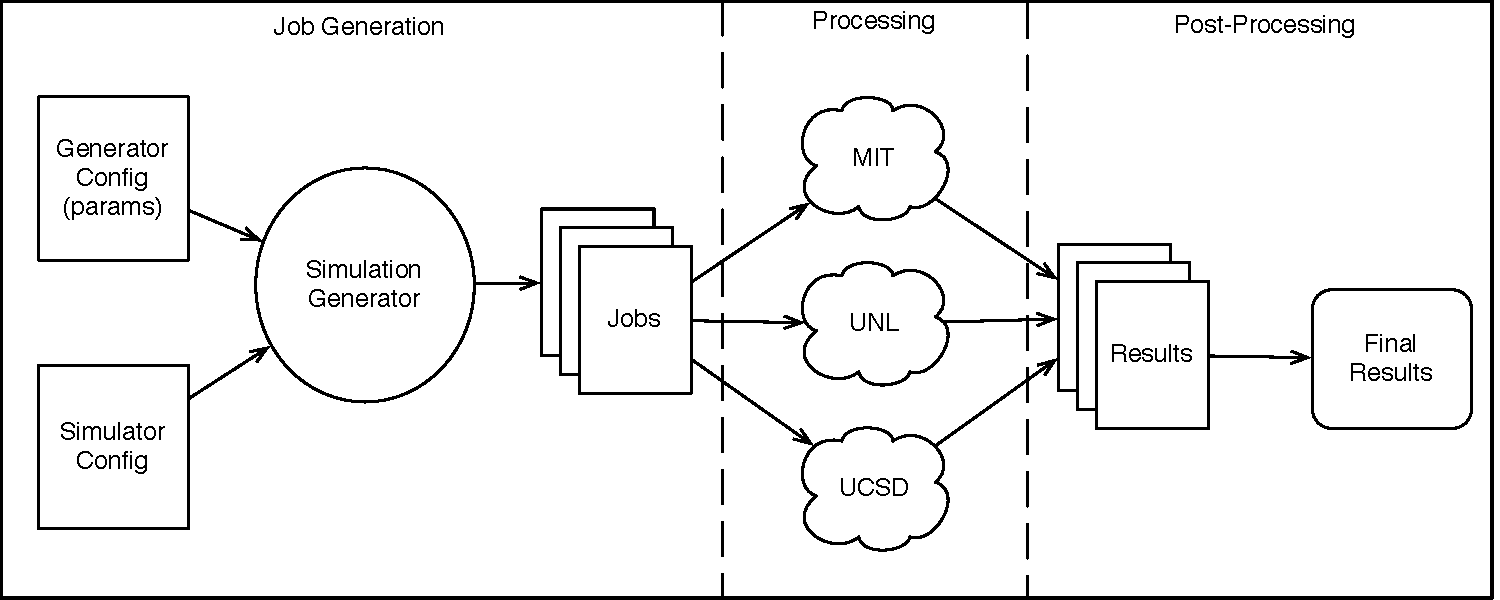
\includegraphics[width=\textwidth]{images/ProcessOverview}
\caption{Overview of Simulation Processing}
\label{fig:processoverview}
\end{figure*}

\subsection{Job Generation}
\label{sec:jobgeneration}
The simulation generator takes two input files.  The first is the simulation configuration file, and the second is the Generator Configuration file, a file describing the range of values that simulation values should take.

The configuration file is a standard configuration file describing the simulation parameters.  The only difference is values that will be replaced in the file are specified with a special qualifier.  The format of the qualifier is: \texttt{\%($<$name$>$)s}, where \texttt{name} is a unique name that corresponds to the name given in the generator configuration file.  

The simulation configuration file consists of key/value pairs describing how each variable should be replaced in the simulation configuration.  The keys correspond to the \texttt{name} given in the simulation configuration file.  The values are explicitly formatted to define the range of values that the variables are to be set in the generated simulation files.  


\begin{figure}[ht]
\lstset{ frame=single}
\begin{lstlisting}
[main]
param = [1.0..2.0] step 1
repeat_param = [1..10] step 4 repeat 10
\end{lstlisting}
\caption{Example generator configuration file}
\label{fig:simgenexample}
\end{figure}

Example values are shown in Figure \ref{fig:simgenexample}.  In this example, there is a parameter, \texttt{param}, that iterates from $1.0$ to $2.0$, stepping every 1.  In the generated simulation files, \texttt{\%$<$param$>$)} will be replaced with 1.0, and in another simulation file it will be 2.0.

The next parameter in the example Figure \ref{fig:simgenexample} is called \texttt{repeat\_param}.  This parameter has an optional argument after the definition of the range, \texttt{repeat 10}.  This additional argument means that for each possible value of \texttt{repeat\_param}, it should be repeated 10 times.  For example, the first possible value will be 1.  The value of 1 will be in the next 10 simulation files as well.  The next value of \texttt{repeat\_param} will be 5, and it will also be repeated for 10 simulation files.  The next value is 9, repeated 10 times.  Then it rolls over back to 1, repeated 10 times ...

\subsection{Processing}
Remote execution of the simulator is managed by the high throughput resource management system Condor.  The generator creates a Condor submission file that is used to describe the job.  A submission script example is shown in Figure \ref{fig:condorsubmission}.  The submission script describes the job with lines such as which \texttt{executable} to run on the remote host, and \texttt{transfer\_input\_files} specifies what input files to transfer to the remote host before starting the \texttt{executable}.  The \texttt{output} and \texttt{error} specify files that have the stdout and stderr (respectively) of the executable.

\begin{figure} [ht]
\lstset{ frame=single,
breaklines=true,                % sets automatic line breaking
breakatwhitespace=true }
\begin{lstlisting}
should_transfer_files = YES
executable = share/submission.sh
transfer_input_files = tcl8.4.11.tar.gz,\
   ns, \ 
   output3/submit0.simconfig
log = condor.log
when_to_transfer_output = ON_EXIT
universe = vanilla
arguments = output3/submit0.simconfig
error = output3/submit0.simconfig.err
output = output3/submit0.simconfig.out
queue
\end{lstlisting}
\caption{Example submission file generated by }
\label{fig:condorsubmission}
\end{figure}

When the job is submitted to Condor, it will manage the execution of the job until completion.  First it will send a request to the central manager for nodes to run on.  After receiving confirmation of a available node, it will contact the worker node and begin transferring files.  The transferred files are those specified by the \texttt{transfer\_input\_files}, plus the executable.  Once the transfers are completed, Condor will begin the executable.  

The executable is a custom shell script distributed with our project.  It will first uncompress the NS-2 simulator and the tcl version that NS depends on.  The script will execute the simulation using the simulation configuration that was given to the the executable as the \texttt{arguments}.


% Independent variables


\section{Evaluation}

\subsection{Simulation}
We designed a simulated Wireless Sensor Network using Network Simulator(NS-2) and Mannasim\cite{braga2004mannasim} patch. NS-2 is a general simulator tool used for simulation of any kind of wired or wireless networks. The wireless sensor networks which we are interested in are implemented using the Mannsim patch. 

In the original simulation configuration, the simulated WSN has nodes with all possible links among themselves excepting for self loops. All the links have 1Mb of bandwidth and the packet size is 500 bytes. Packets are transmitted from Node 1 and Node 2 at an interval of 0.005 units of time and node 20 is the receiver of the routed packets. In order to replicate the real WSN scenario the link between some pairs of nodes are turned off, being restored after 1 min in simulation time. 

\subsection{Experimental Design}
The original simulation configuration was modified such that 4 variables where replaced and iterated using the simulation generator.  The variables in the NS-2 configuration where specified with the special qualifier specified in the Section \label{sec:jobgeneration}.  A snippet of the NS-2 configuration file showing two of the variables replaces is shown in Figure \ref{fig:ns2experimentconf}.

\begin{figure}[ht]
\lstset{ frame=single,
breaklines=true,                % sets automatic line breaking
breakatwhitespace=true }
\begin{lstlisting}
set udp0 [new Agent/UDP]
#udp is the link protocol
$ns attach-agent $n(0) $udp0
set cbr0 [new Application/Traffic/Exponential]
#cbr is the traffic generator

#set the size of the packet
$cbr0 set packetSize_ %(packetsize05)i
#set the interval after which the packet is sent
$cbr0 set interval_ %(interval05)lf
\end{lstlisting}
\caption{NS-2 Simulation Configuration Variables}
\label{fig:ns2experimentconf}
\end{figure}

Each variable was specified in the simulation generator configuration file as shown in Figure \ref{fig:experimentsimconfig}.  

\begin{figure}[ht]
\lstset{ frame=single,
breaklines=true,                % sets automatic line breaking
breakatwhitespace=true }
\begin{lstlisting}
[main]

packetsize05 = [300..1000] step 100
packetsize15 = [300..1000] step 100

interval05 = [0.001..0.100] step 0.002
interval15 = [0.001..0.100] step 0.002
\end{lstlisting}
\caption{Simulation Configuration from the experiment}
\label{fig:experimentsimconfig}
\end{figure}

The experiment simulations created $117,649$  simulations.  The simulations where submitted to the Open Science Grid,  running over 15 clusters across the U.S.  Figure \ref{fig:allsites} shows the sites that run the evaluation runs.  

\begin{figure*}[ht]
\centering
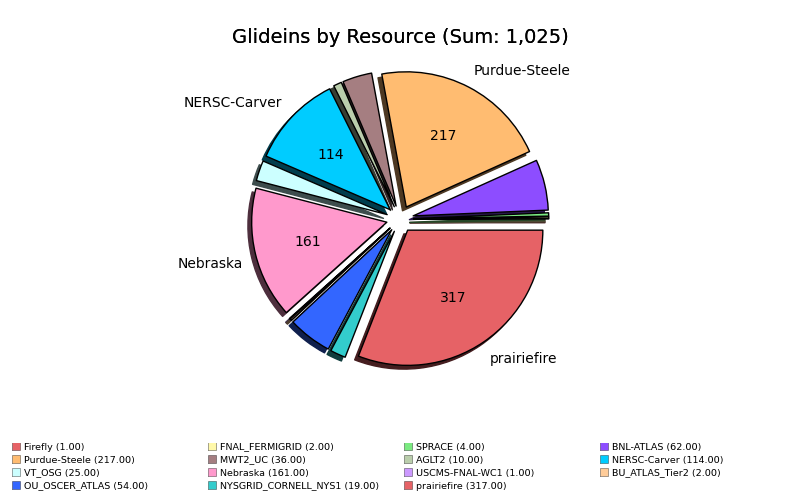
\includegraphics[width=\textwidth]{images/allsites.png}
\caption{An snapshot of the processing sites for the evaluation runs}
\label{fig:allsites}
\end{figure*}


\section{Conclusion}
In this project, we created a framework that manages the simulations of complex network configurations.  The simulation generator creates configurations for the simulator that iterates over interesting variables, simplifying the user's job of creating the simulations.  The simulations are then submitted to a resource manager for execution over an computational cluster or grid, greatly decreasing the amount of time spent simulating the network.  Our network was then evaluated when an example network, and iterating over four variables, creating $117,649$ independent simulations that where executed on the Open Science Grid.




% An example of a floating figure using the graphicx package.
% Note that \label must occur AFTER (or within) \caption.
% For figures, \caption should occur after the \includegraphics.
% Note that IEEEtran v1.7 and later has special internal code that
% is designed to preserve the operation of \label within \caption
% even when the captionsoff option is in effect. However, because
% of issues like this, it may be the safest practice to put all your
% \label just after \caption rather than within \caption{}.
%
% Reminder: the "draftcls" or "draftclsnofoot", not "draft", class
% option should be used if it is desired that the figures are to be
% displayed while in draft mode.
%
%\begin{figure}[!t]
%\centering
%\includegraphics[width=2.5in]{myfigure}
% where an .eps filename suffix will be assumed under latex, 
% and a .pdf suffix will be assumed for pdflatex; or what has been declared
% via \DeclareGraphicsExtensions.
%\caption{Simulation Results}
%\label{fig_sim}
%\end{figure}

% Note that IEEE typically puts floats only at the top, even when this
% results in a large percentage of a column being occupied by floats.


% An example of a double column floating figure using two subfigures.
% (The subfig.sty package must be loaded for this to work.)
% The subfigure \label commands are set within each subfloat command, the
% \label for the overall figure must come after \caption.
% \hfil must be used as a separator to get equal spacing.
% The subfigure.sty package works much the same way, except \subfigure is
% used instead of \subfloat.
%
%\begin{figure*}[!t]
%\centerline{\subfloat[Case I]\includegraphics[width=2.5in]{subfigcase1}%
%\label{fig_first_case}}
%\hfil
%\subfloat[Case II]{\includegraphics[width=2.5in]{subfigcase2}%
%\label{fig_second_case}}}
%\caption{Simulation results}
%\label{fig_sim}
%\end{figure*}
%
% Note that often IEEE papers with subfigures do not employ subfigure
% captions (using the optional argument to \subfloat), but instead will
% reference/describe all of them (a), (b), etc., within the main caption.


% An example of a floating table. Note that, for IEEE style tables, the 
% \caption command should come BEFORE the table. Table text will default to
% \footnotesize as IEEE normally uses this smaller font for tables.
% The \label must come after \caption as always.
%
%\begin{table}[!t]
%% increase table row spacing, adjust to taste
%\renewcommand{\arraystretch}{1.3}
% if using array.sty, it might be a good idea to tweak the value of
% \extrarowheight as needed to properly center the text within the cells
%\caption{An Example of a Table}
%\label{table_example}
%\centering
%% Some packages, such as MDW tools, offer better commands for making tables
%% than the plain LaTeX2e tabular which is used here.
%\begin{tabular}{|c||c|}
%\hline
%One & Two\\
%\hline
%Three & Four\\
%\hline
%\end{tabular}
%\end{table}


% Note that IEEE does not put floats in the very first column - or typically
% anywhere on the first page for that matter. Also, in-text middle ("here")
% positioning is not used. Most IEEE journals/conferences use top floats
% exclusively. Note that, LaTeX2e, unlike IEEE journals/conferences, places
% footnotes above bottom floats. This can be corrected via the \fnbelowfloat
% command of the stfloats package.




% conference papers do not normally have an appendix


% use section* for acknowledgement
%\section*{Acknowledgment}


%The authors would like to thank...





% trigger a \newpage just before the given reference
% number - used to balance the columns on the last page
% adjust value as needed - may need to be readjusted if
% the document is modified later
%\IEEEtriggeratref{8}
% The "triggered" command can be changed if desired:
%\IEEEtriggercmd{\enlargethispage{-5in}}

% references section

% can use a bibliography generated by BibTeX as a .bbl file
% BibTeX documentation can be easily obtained at:
% http://www.ctan.org/tex-archive/biblio/bibtex/contrib/doc/
% The IEEEtran BibTeX style support page is at:
% http://www.michaelshell.org/tex/ieeetran/bibtex/
\bibliographystyle{IEEEtran}
% argument is your BibTeX string definitions and bibliography database(s)
\bibliography{project}
%
% <OR> manually copy in the resultant .bbl file
% set second argument of \begin to the number of references
% (used to reserve space for the reference number labels box)




% that's all folks
\end{document}


